\chapter{Mod�le du syst�me}

Etudions maintenant les possibilit�s d'utilisation du futur logiciel.

\section{Cas d'utilisation}

\begin{figure}[h!t]
  \centering
  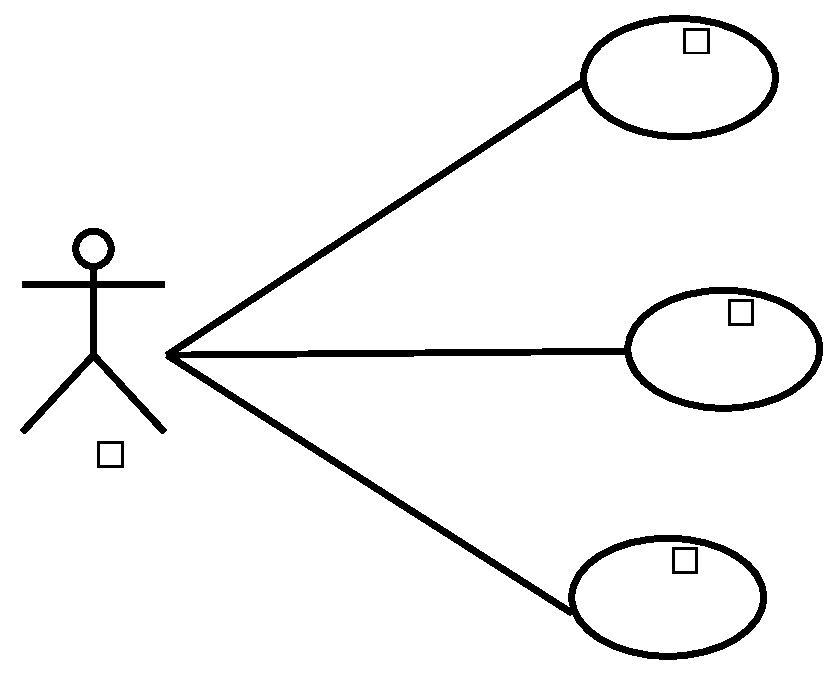
\includegraphics{simple}
  \caption{Diagramme des Uses Case simple}
  \label{fig:diagramme_simple}
\end{figure}

\begin{figure}[h!t]
  \centering
  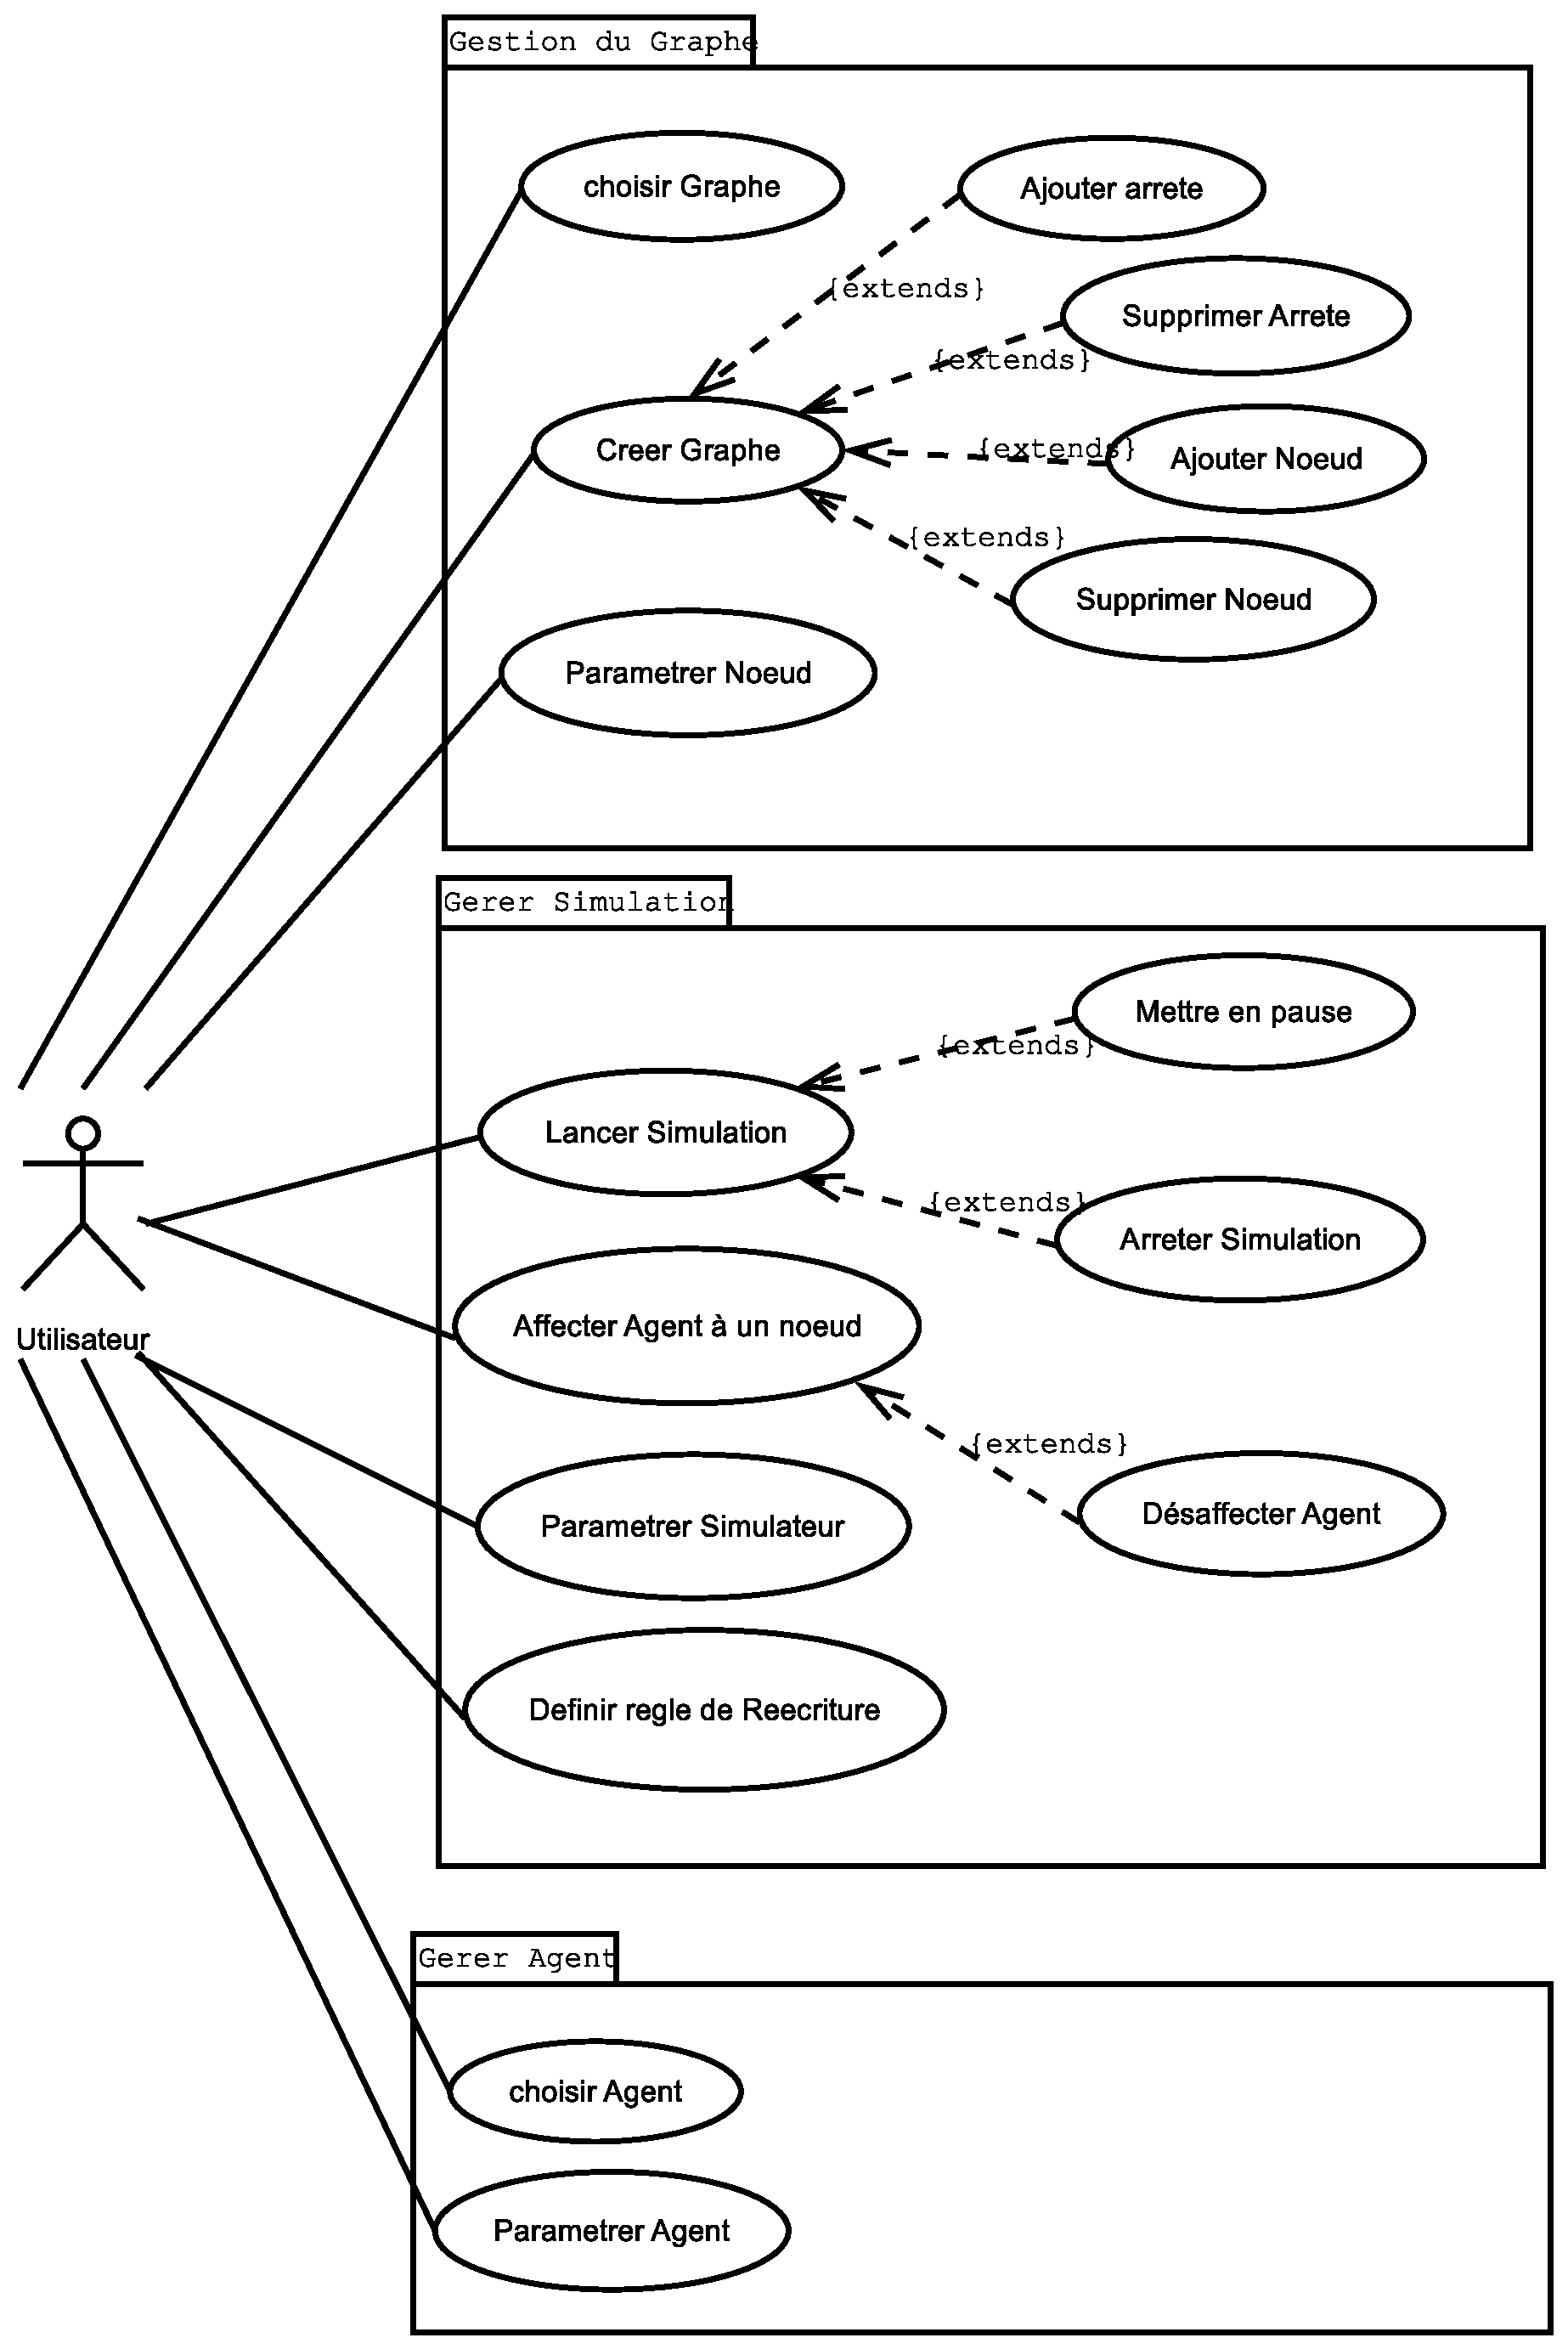
\includegraphics[width=14cm]{UseCase}  
  \caption{Diagramme des Uses Case}
  \label{fig:diagramme_UseCase}
\end{figure}


\subsection{D�finir r�gles de r��criture}

Ce cas d'utilisation va permettre � l'utilisateur de concevoir un
algorithme de mani�re simplifi�. En effet, l'utilisateur sp�cifie �
l'aide d'une interface graphique le comportement d'un agent par un
ensemble de r�gles, sans devoir le programmer par l'API bas niveau. Ce
cas d'utilisation sera accessible seulement dans la fen�tre
simulation.

%\subsection{Cartouche d'identification de la fiche de cas d'utilisation}

%\begin{table}[ht!]
%\begin{tabular}{|l|l|}
%\hline
%Nom fiche de cas d'utilisation & DefineRewritingRule \\  \hline
%Date de mise a jour & $LastChangedDate$ \\ \hline
%Version & 0.1 \\ \hline
%Redacteur & Xavier\\ \hline
%Priorit� du cas d'utilisation & Moyen \\ \hline
%\end{tabular}
%\caption{} \label{cartouche_ReglesReecriture}
%\end{table}


\subsubsection{G�n�ralit�s}

%\begin{table}[h!t]
\begin{tabular}{|l|p{11cm}|}
    \hline
    Cas d'utilisation & D�finir des r�gles de r��criture. \\ \hline
    Acteurs & L'utilisateur. \\ \hline
    \multirow{2}{0cm}{But} & Permettre � l'utilisateur de d�finir des r�gles de r��criture
    relativement au comportement des agents. \\ \hline
    R�sum� M�tier & L'utilisateur d�finit ses r�gles de r��criture de
    mani�re ``graphique''. \\ \hline
    Pr� conditions & Un graphe est charg� dans le syst�me \\ \hline
    Post conditions & Les r�gles de r��critures sont d�finies. \\ \hline
    Commentaires & Tous les agents utilisent un seul jeu de r�gles de r��criture.\\ \hline
  \end{tabular}
  % \caption{} 
%  \label{genralites_ReglesReecriture}
%\end{table}

\subsubsection{Sc�nario Nominal}

%\begin{table}[h!t]
\begin{tabular}{|c|l|}
\hline
Num�ro encha�nement & Action \\  \hline
1 & L'utilisateur saisit une r�gle de r��criture et valide \\ \hline
2 & Le syst�me enregistre les r�gles de r��criture\\ \hline
\end{tabular}
%\caption{}
%\label{nominal_ReglesReecriture}
%\end{table}

\subsubsection{Sc�nario Alternatif}

%\begin{table}[h!t]
\begin{tabular}{|c|l|}
\hline
N encha�nement & Action \\ \hline
Au point 2: 2.1 & L'utilisateur ajoute une nouvelle r�gle de r��criture\\ \hline
 2.1.1 & L'utilisateur saisit une nouvelle r�gle de r��criture et
 valide \\ \hline
 2.1.2 & Retour au point 1 \\ \hline
Au point 2: 2.2 & L'utilisateur supprime une r�gle de r��criture\\
\hline
 2.2.1 & Retour au point 1 \\ \hline
\end{tabular}
%\caption{}
%\label{alternatif_ReglesReecriture}
%\end{table}


\subsubsection{Exceptions}

Pas de sc�nario d'exception.


\section{Choisir Graphe}
%\subsection{Cartouche d'identification de la fiche de cas d'utilisation}

%\begin{table}[ht!]
%\begin{tabular}{|l|l|}
%\hline
%Nom fiche de cas d'utilisation & OpenGraph \\  \hline
%Date de mise a jour & $LastChangedDate$ \\ \hline
%Version & 0.1 \\ \hline
%Redacteur & Xavier\\ \hline
%Priorit� du cas d'utilisation & Faible \\
%\hline
%\end{tabular}
%\caption{} \label{cartouche_choisirGraphe}
%\end{table}


\subsection{Description du cas d'utilisation}

\subsubsection{G�n�ralit�s}

\begin{table}[ht!]
\begin{tabular}{|l|l|}
\hline
Cas d'utilisation & Choisir un graphe. \\ \hline
Acteurs & L'utilisateur. \\ \hline
But & Permettre � l'utilisateur de sp�cifier le graphe sur lequel on
va travailler. \\ \hline
R�sum� M�tier & L'utilisateur indique le fichier graphe (format GML). \\ \hline
Pr� conditions & L'utilsateur dispose de graphes. \\ \hline
Post conditions & Le graphe est charg�. \\ \hline
Commentaires & Un seul graphe ne peut �tre charger � la fois.\\ \hline
\end{tabular}
%\caption{} 
\label{genralites_choisirGraphe}
\end{table}

\subsubsection{Sc�nario Nominal}

\begin{table}[ht!]
\begin{tabular}{|c|l|}
\hline
Num�ro enchainement & Action \\  \hline
1 & Le syst�me pr�sente le choix des graphes \\ \hline
2 & L'utilisateur s�lectionne le graphe \\ \hline
3 & Le syst�me charge le graphe\\ \hline
\end{tabular}
\caption{} \label{nominal_choisirGraphe}
\end{table}

\subsubsection{Sc�nario Alternatif}

Pas de sc�nario alternatif

\subsubsection{Exceptions}

\begin{table}[ht!]
\begin{tabular}{|l|l|}
\hline
N enchainement & Action \\ \hline
Au point 2: 2.1 & L'utilisateur annule\\ \hline
 2.1.1 & Fin du use case\\ \hline
\end{tabular}
\caption{} \label{exceptions_choisirGraphe}
\end{table}

\section{Choisir Agent}
%\subsection{Cartouche d'identification de la fiche de cas d'utilisation}

%\begin{table}[h!]
%\begin{tabular}{|l|l|}
%\hline
%Nom fiche de cas d'utilisation & OpenAgent \\  \hline
%Date de mise a jour & $LastChangedDate$ \\ \hline
%Version & 0.1 \\ \hline
%Redacteur & Xavier\\ \hline
%Priorit� du cas d'utilisation & Faible \\
%\hline
%\end{tabular}
%\caption{} \label{cartouche_choisirAgent}
%\end{table}


\subsection{Description du cas d'utilisation}

\subsubsection{G�n�ralit�s}

\begin{table}[h!t]
\begin{tabular}{|l|l|}
  \hline
  Cas d'utilisation & Choisir un Agent. \\ \hline
  Acteurs & L'utilisateur. \\ \hline
  But & Permettre � l'utilisateur de sp�cifier les agents qui vont
  op�rer sur le graphe. \\ \hline
  R�sum� M�tier & L'utilisateur indique le fichier agent (format
  byteCode Java). \\ \hline
  Pr� conditions & L'utilsateur dispose d'implantation d'agents. \\ \hline
  Post conditions & L'agent est charg�. \\ \hline
  Commentaires &  Un seule implantation d'agent peut �tre
  s�lectionn�e (l'implantation par d�faut).\\ \hline
\end{tabular}
%\caption{} 
\label{genralites_choisirAgent}
\end{table}

\subsubsection{Sc�nario Nominal}

\begin{table}[h!t]
\begin{tabular}{|c|l|}
\hline
Num�ro enchainement & Action \\  \hline
1 & Le syst�me pr�sente le choix des agents \\ \hline
2 & L'utilisateur s�lectionne l'agent \\ \hline
3 & Le syst�me charge l'agent\\ \hline
\end{tabular}
%\caption{}
\label{nominal_choisirAgent}
\end{table}

\subsubsection{Sc�nario Alternatif}

Pas de sc�nario alternatif

\subsubsection{Exceptions}

\begin{table}[h!t]
\begin{tabular}{|c|l|}
\hline
N enchainement & Action \\ \hline
Au point 2: 2.1 & L'utilisateur annule\\ \hline
 2.1.1 & Fin du use case\\ \hline
\end{tabular}
%\caption{}
\label{exceptions_choisirAgent}
\end{table}



\section{Diagramme de classes}

Notre  projet  s'architecture autour  d'une  classe principale  nomm�e
Agent.  Le diagramme  UML  de  classes est  disponible  sur la  figure
\ref{fig:diagramme_classes}.

\begin{figure}[ht]
  \centering
  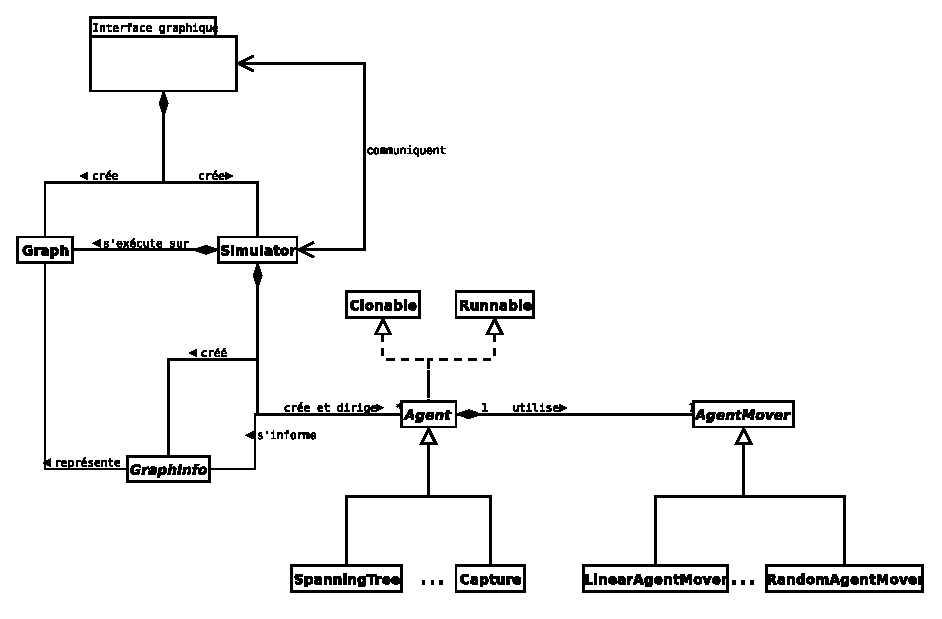
\includegraphics[width=14cm]{classes} 
  \caption{Diagramme de classes}
  \label{fig:diagramme_classes}
\end{figure}

\subsection{La classe Agent et ses sous-classes}

La  classe  Agent  impl�mente  toutes les  m�thodes  n�cessaires  pour
faciliter  le  travail du  futur  d�veloppeur  d'agents mobiles.   Les
m�thodes  seront  d�crites dans  la  partie  \ref{sec:api}  � la  page
\pageref{sec:api}. \\

De fa�on g�n�rale, on peut  trouver des m�thodes d'informations sur le
graphe, des m�thodes  de gestion de propri�t�s (au  niveau des sommets
et des portes), des m�thodes de d�placements et de clonage.\\

Le futur d�veloppeur devra,  pour impl�menter ses agents, sous-classer
cette classe Agent et impl�menter la m�thode abstraite suivante : \\

\begin{description}
\item[init] Utilis�e pour impl�menter le code g�n�ral de l'algorithme.
  C'est cette m�thode qui sera lanc�e lorsque l'agent sera ex�cut�.
\end{description}

\subsection{La classe AgentMover}

AgentMover  est  une classe  qui  a pour  but  d'apporter  un type  de
d�placement aux  agents. Certains type de  d�placements seront fournis
par \visidia et d'autres  pourront �tre impl�ment�s par le d�veloppeur
lorsqu'il en ressentira le besoin. \\

Lors de l'impl�mentation d'un agent, le d�veloppeur devra utiliser les
m�thodes  ``move'' pour  se d�placer.  Ces m�thodes  sont en  fait des
appels cach�s aux m�thodes de AgentMover. \\

Pour d�velopper  un nouveau  type de d�placement,  l'utilisateur devra
donc impl�menter  une nouvelle sous classe de  AgentMover et red�finir
la m�thode ``findNextDoor''.

%% Local Variables:
%% mode: latex
%% coding: latin-1
%% TeX-master: "main"
%% End:
